\documentclass[tikz,border=5pt]{standalone}
\usepackage[T1]{fontenc}
\usepackage{lmodern,amsmath,amssymb}
\usetikzlibrary{arrows.meta,calc,positioning,fit,backgrounds,shapes.geometric,matrix,decorations.pathreplacing,patterns}
\definecolor{ink}{gray}{0.08}
\definecolor{wash}{gray}{0.965}
\definecolor{soft}{gray}{0.45}
\tikzset{box/.style={draw=ink,line width=.65pt,fill=white,align=center,inner sep=4pt,outer sep=0pt,font=\small},flow/.style={draw=ink,line width=.65pt,-{Latex[length=1.8mm,width=1.3mm]},rounded corners=2pt},annotation/.style={font=\scriptsize,text=soft,align=center},groupbox/.style={draw=soft,dashed,line width=.45pt,fill=wash}}
\begin{document}
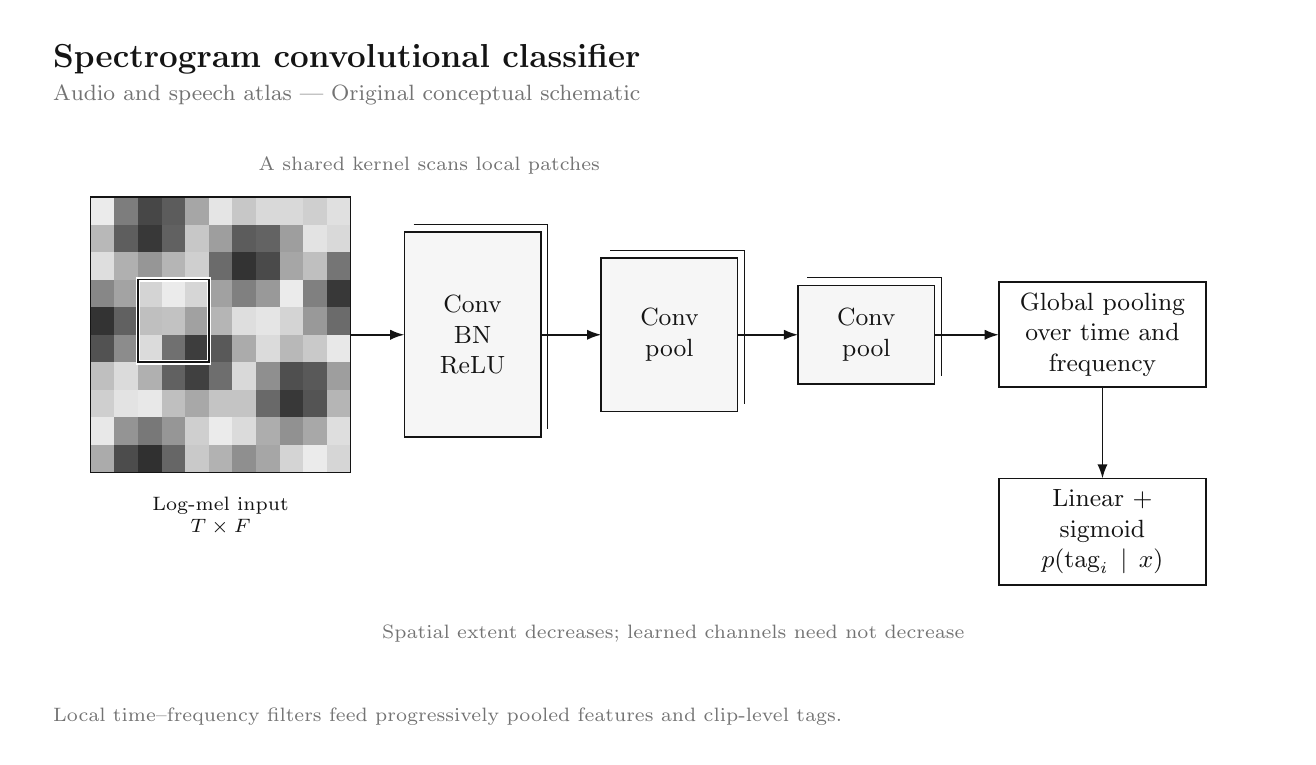
\begin{tikzpicture}[x=1cm,y=-1cm,font=\rmfamily,text=ink]

\path[use as bounding box] (0,0) rectangle (16,9);
\node[anchor=west,font=\large\bfseries] at (.2,.4) {Spectrogram convolutional classifier};
\node[anchor=west,font=\footnotesize,text=soft] at (.2,.85) {Audio and speech atlas | Original conceptual schematic};
\begin{pgfonlayer}{background}
\end{pgfonlayer}
\node[align=center,inner sep=0pt,outer sep=0pt,font=\small,minimum width=3.3cm,minimum height=3.5cm,text width=3.05cm] (spec) at (2.45,3.9) {};
\node[box,fill=wash,minimum width=1.7cm,minimum height=2.6cm,text width=1.45cm] (conv1) at (5.65,3.9) {Conv\\BN\\ReLU};
\draw[ink,line width=.4pt] (4.9,2.4999999999999996) -- (6.6,2.4999999999999996) -- (6.6,5.1000000000000005);
\node[box,fill=wash,minimum width=1.7cm,minimum height=1.95cm,text width=1.45cm] (conv2) at (8.15,3.9) {Conv\\pool};
\draw[ink,line width=.4pt] (7.4,2.8249999999999997) -- (9.1,2.8249999999999997) -- (9.1,4.775);
\node[box,fill=wash,minimum width=1.7cm,minimum height=1.25cm,text width=1.45cm] (conv3) at (10.65,3.9) {Conv\\pool};
\draw[ink,line width=.4pt] (9.9,3.175) -- (11.6,3.175) -- (11.6,4.425000000000001);
\node[box,minimum width=2.6cm,minimum height=1.15cm,text width=2.35cm] (global) at (13.65,3.9) {Global pooling\\over time and frequency};
\node[box,minimum width=2.6cm,minimum height=1.05cm,text width=2.35cm] (tags) at (13.65,6.4) {Linear + sigmoid\\$p(\text{tag}_i\mid x)$};
\begin{pgfonlayer}{background}
\draw[flow] (spec.east) -- (conv1.west);
\draw[flow] (conv1.east) -- (conv2.west);
\draw[flow] (conv2.east) -- (conv3.west);
\draw[flow] (conv3.east) -- (global.west);
\draw[flow] (global.south) -- (tags.north);
\end{pgfonlayer}
\fill[black!8] (0.800,2.150) rectangle (1.100,2.500);
\fill[black!28] (0.800,2.500) rectangle (1.100,2.850);
\fill[black!13] (0.800,2.850) rectangle (1.100,3.200);
\fill[black!47] (0.800,3.200) rectangle (1.100,3.550);
\fill[black!80] (0.800,3.550) rectangle (1.100,3.900);
\fill[black!68] (0.800,3.900) rectangle (1.100,4.250);
\fill[black!25] (0.800,4.250) rectangle (1.100,4.600);
\fill[black!19] (0.800,4.600) rectangle (1.100,4.950);
\fill[black!9] (0.800,4.950) rectangle (1.100,5.300);
\fill[black!33] (0.800,5.300) rectangle (1.100,5.650);
\fill[black!51] (1.100,2.150) rectangle (1.400,2.500);
\fill[black!63] (1.100,2.500) rectangle (1.400,2.850);
\fill[black!31] (1.100,2.850) rectangle (1.400,3.200);
\fill[black!36] (1.100,3.200) rectangle (1.400,3.550);
\fill[black!62] (1.100,3.550) rectangle (1.400,3.900);
\fill[black!45] (1.100,3.900) rectangle (1.400,4.250);
\fill[black!14] (1.100,4.250) rectangle (1.400,4.600);
\fill[black!11] (1.100,4.600) rectangle (1.400,4.950);
\fill[black!42] (1.100,4.950) rectangle (1.400,5.300);
\fill[black!70] (1.100,5.300) rectangle (1.400,5.650);
\fill[black!72] (1.400,2.150) rectangle (1.700,2.500);
\fill[black!78] (1.400,2.500) rectangle (1.700,2.850);
\fill[black!41] (1.400,2.850) rectangle (1.700,3.200);
\fill[black!17] (1.400,3.200) rectangle (1.700,3.550);
\fill[black!25] (1.400,3.550) rectangle (1.700,3.900);
\fill[black!14] (1.400,3.900) rectangle (1.700,4.250);
\fill[black!31] (1.400,4.250) rectangle (1.700,4.600);
\fill[black!9] (1.400,4.600) rectangle (1.700,4.950);
\fill[black!53] (1.400,4.950) rectangle (1.700,5.300);
\fill[black!81] (1.400,5.300) rectangle (1.700,5.650);
\fill[black!64] (1.700,2.150) rectangle (2.000,2.500);
\fill[black!62] (1.700,2.500) rectangle (2.000,2.850);
\fill[black!29] (1.700,2.850) rectangle (2.000,3.200);
\fill[black!8] (1.700,3.200) rectangle (2.000,3.550);
\fill[black!24] (1.700,3.550) rectangle (2.000,3.900);
\fill[black!56] (1.700,3.900) rectangle (2.000,4.250);
\fill[black!62] (1.700,4.250) rectangle (2.000,4.600);
\fill[black!25] (1.700,4.600) rectangle (2.000,4.950);
\fill[black!41] (1.700,4.950) rectangle (2.000,5.300);
\fill[black!60] (1.700,5.300) rectangle (2.000,5.650);
\fill[black!35] (2.000,2.150) rectangle (2.300,2.500);
\fill[black!22] (2.000,2.500) rectangle (2.300,2.850);
\fill[black!19] (2.000,2.850) rectangle (2.300,3.200);
\fill[black!16] (2.000,3.200) rectangle (2.300,3.550);
\fill[black!37] (2.000,3.550) rectangle (2.300,3.900);
\fill[black!76] (2.000,3.900) rectangle (2.300,4.250);
\fill[black!75] (2.000,4.250) rectangle (2.300,4.600);
\fill[black!34] (2.000,4.600) rectangle (2.300,4.950);
\fill[black!19] (2.000,4.950) rectangle (2.300,5.300);
\fill[black!21] (2.000,5.300) rectangle (2.300,5.650);
\fill[black!10] (2.300,2.150) rectangle (2.600,2.500);
\fill[black!38] (2.300,2.500) rectangle (2.600,2.850);
\fill[black!58] (2.300,2.850) rectangle (2.600,3.200);
\fill[black!37] (2.300,3.200) rectangle (2.600,3.550);
\fill[black!29] (2.300,3.550) rectangle (2.600,3.900);
\fill[black!65] (2.300,3.900) rectangle (2.600,4.250);
\fill[black!57] (2.300,4.250) rectangle (2.600,4.600);
\fill[black!23] (2.300,4.600) rectangle (2.600,4.950);
\fill[black!8] (2.300,4.950) rectangle (2.600,5.300);
\fill[black!30] (2.300,5.300) rectangle (2.600,5.650);
\fill[black!22] (2.600,2.150) rectangle (2.900,2.500);
\fill[black!64] (2.600,2.500) rectangle (2.900,2.850);
\fill[black!80] (2.600,2.850) rectangle (2.900,3.200);
\fill[black!50] (2.600,3.200) rectangle (2.900,3.550);
\fill[black!13] (2.600,3.550) rectangle (2.900,3.900);
\fill[black!33] (2.600,3.900) rectangle (2.900,4.250);
\fill[black!15] (2.600,4.250) rectangle (2.900,4.600);
\fill[black!23] (2.600,4.600) rectangle (2.900,4.950);
\fill[black!14] (2.600,4.950) rectangle (2.900,5.300);
\fill[black!44] (2.600,5.300) rectangle (2.900,5.650);
\fill[black!15] (2.900,2.150) rectangle (3.200,2.500);
\fill[black!61] (2.900,2.500) rectangle (3.200,2.850);
\fill[black!71] (2.900,2.850) rectangle (3.200,3.200);
\fill[black!40] (2.900,3.200) rectangle (3.200,3.550);
\fill[black!10] (2.900,3.550) rectangle (3.200,3.900);
\fill[black!14] (2.900,3.900) rectangle (3.200,4.250);
\fill[black!44] (2.900,4.250) rectangle (3.200,4.600);
\fill[black!59] (2.900,4.600) rectangle (3.200,4.950);
\fill[black!32] (2.900,4.950) rectangle (3.200,5.300);
\fill[black!35] (2.900,5.300) rectangle (3.200,5.650);
\fill[black!15] (3.200,2.150) rectangle (3.500,2.500);
\fill[black!38] (3.200,2.500) rectangle (3.500,2.850);
\fill[black!35] (3.200,2.850) rectangle (3.500,3.200);
\fill[black!8] (3.200,3.200) rectangle (3.500,3.550);
\fill[black!17] (3.200,3.550) rectangle (3.500,3.900);
\fill[black!28] (3.200,3.900) rectangle (3.500,4.250);
\fill[black!69] (3.200,4.250) rectangle (3.500,4.600);
\fill[black!78] (3.200,4.600) rectangle (3.500,4.950);
\fill[black!43] (3.200,4.950) rectangle (3.500,5.300);
\fill[black!17] (3.200,5.300) rectangle (3.500,5.650);
\fill[black!19] (3.500,2.150) rectangle (3.800,2.500);
\fill[black!11] (3.500,2.500) rectangle (3.800,2.850);
\fill[black!25] (3.500,2.850) rectangle (3.800,3.200);
\fill[black!50] (3.500,3.200) rectangle (3.800,3.550);
\fill[black!40] (3.500,3.550) rectangle (3.800,3.900);
\fill[black!21] (3.500,3.900) rectangle (3.800,4.250);
\fill[black!65] (3.500,4.250) rectangle (3.800,4.600);
\fill[black!67] (3.500,4.600) rectangle (3.800,4.950);
\fill[black!34] (3.500,4.950) rectangle (3.800,5.300);
\fill[black!8] (3.500,5.300) rectangle (3.800,5.650);
\fill[black!12] (3.800,2.150) rectangle (4.100,2.500);
\fill[black!15] (3.800,2.500) rectangle (4.100,2.850);
\fill[black!54] (3.800,2.850) rectangle (4.100,3.200);
\fill[black!78] (3.800,3.200) rectangle (4.100,3.550);
\fill[black!58] (3.800,3.550) rectangle (4.100,3.900);
\fill[black!9] (3.800,3.900) rectangle (4.100,4.250);
\fill[black!38] (3.800,4.250) rectangle (4.100,4.600);
\fill[black!29] (3.800,4.600) rectangle (4.100,4.950);
\fill[black!13] (3.800,4.950) rectangle (4.100,5.300);
\fill[black!16] (3.800,5.300) rectangle (4.100,5.650);
\draw[ink,line width=.5pt] (0.8,2.15) rectangle (4.1,5.65);
\draw[white,line width=1.6pt] (1.4,3.2) rectangle (2.3,4.25);\draw[ink,line width=.6pt] (1.4,3.2) rectangle (2.3,4.25);
\node[align=center,anchor=center,font=\scriptsize,text=ink,text width=3.5cm] at (2.45,6.2) {Log-mel input\\\mbox{$T\times F$}};
\node[align=center,anchor=center,font=\scriptsize,text=soft,text width=5cm] at (5.1,1.75) {A shared kernel scans local patches};
\node[align=center,anchor=center,font=\scriptsize,text=soft,text width=10cm] at (8.2,7.7) {Spatial extent decreases; learned channels need not decrease};
\node[anchor=west,align=left,font=\scriptsize,text=soft,text width=15.6cm] at (.2,8.75) {Local time--frequency filters feed progressively pooled features and clip-level tags.};
\end{tikzpicture}
\end{document}
